
%% bare_jrnl.tex
%% V1.3
%% 2007/01/11
%% by Michael Shell
%% see http://www.michaelshell.org/
%% for current contact information.
%%
%% This is a skeleton file demonstrating the use of IEEEtran.cls
%% (requires IEEEtran.cls version 1.7 or later) with an IEEE journal paper.
%%
%% Support sites:
%% http://www.michaelshell.org/tex/ieeetran/
%% http://www.ctan.org/tex-archive/macros/latex/contrib/IEEEtran/
%% and
%% http://www.ieee.org/



% *** Authors should verify (and, if needed, correct) their LaTeX system  ***
% *** with the testflow diagnostic prior to trusting their LaTeX platform ***
% *** with production work. IEEE's font choices can trigger bugs that do  ***
% *** not appear when using other class files.                            ***
% The testflow support page is at:
% http://www.michaelshell.org/tex/testflow/


%%*************************************************************************
%% Legal Notice:
%% This code is offered as-is without any warranty either expressed or
%% implied; without even the implied warranty of MERCHANTABILITY or
%% FITNESS FOR A PARTICULAR PURPOSE! 
%% User assumes all risk.
%% In no event shall IEEE or any contributor to this code be liable for
%% any damages or losses, including, but not limited to, incidental,
%% consequential, or any other damages, resulting from the use or misuse
%% of any information contained here.
%%
%% All comments are the opinions of their respective authors and are not
%% necessarily endorsed by the IEEE.
%%
%% This work is distributed under the LaTeX Project Public License (LPPL)
%% ( http://www.latex-project.org/ ) version 1.3, and may be freely used,
%% distributed and modified. A copy of the LPPL, version 1.3, is included
%% in the base LaTeX documentation of all distributions of LaTeX released
%% 2003/12/01 or later.
%% Retain all contribution notices and credits.
%% ** Modified files should be clearly indicated as such, including  **
%% ** renaming them and changing author support contact information. **
%%
%% File list of work: IEEEtran.cls, IEEEtran_HOWTO.pdf, bare_adv.tex,
%%                    bare_conf.tex, bare_jrnl.tex, bare_jrnl_compsoc.tex
%%*************************************************************************

% Note that the a4paper option is mainly intended so that authors in
% countries using A4 can easily print to A4 and see how their papers will
% look in print - the typesetting of the document will not typically be
% affected with changes in paper size (but the bottom and side margins will).
% Use the testflow package mentioned above to verify correct handling of
% both paper sizes by the user's LaTeX system.
%
% Also note that the "draftcls" or "draftclsnofoot", not "draft", option
% should be used if it is desired that the figures are to be displayed in
% draft mode.
%
\documentclass[journal]{IEEEtran}
\usepackage{blindtext}
\usepackage{graphicx}

% Some very useful LaTeX packages include:
% (uncomment the ones you want to load)


% *** MISC UTILITY PACKAGES ***
%
%\usepackage{ifpdf}
% Heiko Oberdiek's ifpdf.sty is very useful if you need conditional
% compilation based on whether the output is pdf or dvi.
% usage:
% \ifpdf
%   % pdf code
% \else
%   % dvi code
% \fi
% The latest version of ifpdf.sty can be obtained from:
% http://www.ctan.org/tex-archive/macros/latex/contrib/oberdiek/
% Also, note that IEEEtran.cls V1.7 and later provides a builtin
% \ifCLASSINFOpdf conditional that works the same way.
% When switching from latex to pdflatex and vice-versa, the compiler may
% have to be run twice to clear warning/error messages.






% *** CITATION PACKAGES ***
%
%\usepackage{cite}
% cite.sty was written by Donald Arseneau
% V1.6 and later of IEEEtran pre-defines the format of the cite.sty package
% \cite{} output to follow that of IEEE. Loading the cite package will
% result in citation numbers being automatically sorted and properly
% "compressed/ranged". e.g., [1], [9], [2], [7], [5], [6] without using
% cite.sty will become [1], [2], [5]--[7], [9] using cite.sty. cite.sty's
% \cite will automatically add leading space, if needed. Use cite.sty's
% noadjust option (cite.sty V3.8 and later) if you want to turn this off.
% cite.sty is already installed on most LaTeX systems. Be sure and use
% version 4.0 (2003-05-27) and later if using hyperref.sty. cite.sty does
% not currently provide for hyperlinked citations.
% The latest version can be obtained at:
% http://www.ctan.org/tex-archive/macros/latex/contrib/cite/
% The documentation is contained in the cite.sty file itself.






% *** GRAPHICS RELATED PACKAGES ***
%
\ifCLASSINFOpdf
  % \usepackage[pdftex]{graphicx}
  % declare the path(s) where your graphic files are
  % \graphicspath{{../pdf/}{../jpeg/}}
  % and their extensions so you won't have to specify these with
  % every instance of \includegraphics
  % \DeclareGraphicsExtensions{.pdf,.jpeg,.png}
\else
  % or other class option (dvipsone, dvipdf, if not using dvips). graphicx
  % will default to the driver specified in the system graphics.cfg if no
  % driver is specified.
  % \usepackage[dvips]{graphicx}
  % declare the path(s) where your graphic files are
  % \graphicspath{{../eps/}}
  % and their extensions so you won't have to specify these with
  % every instance of \includegraphics
  % \DeclareGraphicsExtensions{.eps}
\fi
% graphicx was written by David Carlisle and Sebastian Rahtz. It is
% required if you want graphics, photos, etc. graphicx.sty is already
% installed on most LaTeX systems. The latest version and documentation can
% be obtained at: 
% http://www.ctan.org/tex-archive/macros/latex/required/graphics/
% Another good source of documentation is "Using Imported Graphics in
% LaTeX2e" by Keith Reckdahl which can be found as epslatex.ps or
% epslatex.pdf at: http://www.ctan.org/tex-archive/info/
%
% latex, and pdflatex in dvi mode, support graphics in encapsulated
% postscript (.eps) format. pdflatex in pdf mode supports graphics
% in .pdf, .jpeg, .png and .mps (metapost) formats. Users should ensure
% that all non-photo figures use a vector format (.eps, .pdf, .mps) and
% not a bitmapped formats (.jpeg, .png). IEEE frowns on bitmapped formats
% which can result in "jaggedy"/blurry rendering of lines and letters as
% well as large increases in file sizes.
%
% You can find documentation about the pdfTeX application at:
% http://www.tug.org/applications/pdftex


%URL package for url links in the bibliography
\usepackage{url}


% *** MATH PACKAGES ***
%
\usepackage[cmex10]{amsmath}
\usepackage{bm}
% A popular package from the American Mathematical Society that provides
% many useful and powerful commands for dealing with mathematics. If using
% it, be sure to load this package with the cmex10 option to ensure that
% only type 1 fonts will utilized at all point sizes. Without this option,
% it is possible that some math symbols, particularly those within
% footnotes, will be rendered in bitmap form which will result in a
% document that can not be IEEE Xplore compliant!
%
% Also, note that the amsmath package sets \interdisplaylinepenalty to 10000
% thus preventing page breaks from occurring within multiline equations. Use:
\interdisplaylinepenalty=2500
% after loading amsmath to restore such page breaks as IEEEtran.cls normally
% does. amsmath.sty is already installed on most LaTeX systems. The latest
% version and documentation can be obtained at:
% http://www.ctan.org/tex-archive/macros/latex/required/amslatex/math/





% *** SPECIALIZED LIST PACKAGES ***
%
%\usepackage{algorithmic}
% algorithmic.sty was written by Peter Williams and Rogerio Brito.
% This package provides an algorithmic environment fo describing algorithms.
% You can use the algorithmic environment in-text or within a figure
% environment to provide for a floating algorithm. Do NOT use the algorithm
% floating environment provided by algorithm.sty (by the same authors) or
% algorithm2e.sty (by Christophe Fiorio) as IEEE does not use dedicated
% algorithm float types and packages that provide these will not provide
% correct IEEE style captions. The latest version and documentation of
% algorithmic.sty can be obtained at:
% http://www.ctan.org/tex-archive/macros/latex/contrib/algorithms/
% There is also a support site at:
% http://algorithms.berlios.de/index.html
% Also of interest may be the (relatively newer and more customizable)
% algorithmicx.sty package by Szasz Janos:
% http://www.ctan.org/tex-archive/macros/latex/contrib/algorithmicx/




% *** ALIGNMENT PACKAGES ***
%
%\usepackage{array}
% Frank Mittelbach's and David Carlisle's array.sty patches and improves
% the standard LaTeX2e array and tabular environments to provide better
% appearance and additional user controls. As the default LaTeX2e table
% generation code is lacking to the point of almost being broken with
% respect to the quality of the end results, all users are strongly
% advised to use an enhanced (at the very least that provided by array.sty)
% set of table tools. array.sty is already installed on most systems. The
% latest version and documentation can be obtained at:
% http://www.ctan.org/tex-archive/macros/latex/required/tools/


%\usepackage{mdwmath}
%\usepackage{mdwtab}
% Also highly recommended is Mark Wooding's extremely powerful MDW tools,
% especially mdwmath.sty and mdwtab.sty which are used to format equations
% and tables, respectively. The MDWtools set is already installed on most
% LaTeX systems. The lastest version and documentation is available at:
% http://www.ctan.org/tex-archive/macros/latex/contrib/mdwtools/


% IEEEtran contains the IEEEeqnarray family of commands that can be used to
% generate multiline equations as well as matrices, tables, etc., of high
% quality.


%\usepackage{eqparbox}
% Also of notable interest is Scott Pakin's eqparbox package for creating
% (automatically sized) equal width boxes - aka "natural width parboxes".
% Available at:
% http://www.ctan.org/tex-archive/macros/latex/contrib/eqparbox/





% *** SUBFIGURE PACKAGES ***
%\usepackage[tight,footnotesize]{subfigure}
% subfigure.sty was written by Steven Douglas Cochran. This package makes it
% easy to put subfigures in your figures. e.g., "Figure 1a and 1b". For IEEE
% work, it is a good idea to load it with the tight package option to reduce
% the amount of white space around the subfigures. subfigure.sty is already
% installed on most LaTeX systems. The latest version and documentation can
% be obtained at:
% http://www.ctan.org/tex-archive/obsolete/macros/latex/contrib/subfigure/
% subfigure.sty has been superceeded by subfig.sty.



%\usepackage[caption=false]{caption}
%\usepackage[font=footnotesize]{subfig}
% subfig.sty, also written by Steven Douglas Cochran, is the modern
% replacement for subfigure.sty. However, subfig.sty requires and
% automatically loads Axel Sommerfeldt's caption.sty which will override
% IEEEtran.cls handling of captions and this will result in nonIEEE style
% figure/table captions. To prevent this problem, be sure and preload
% caption.sty with its "caption=false" package option. This is will preserve
% IEEEtran.cls handing of captions. Version 1.3 (2005/06/28) and later 
% (recommended due to many improvements over 1.2) of subfig.sty supports
% the caption=false option directly:
%\usepackage[caption=false,font=footnotesize]{subfig}
%
% The latest version and documentation can be obtained at:
% http://www.ctan.org/tex-archive/macros/latex/contrib/subfig/
% The latest version and documentation of caption.sty can be obtained at:
% http://www.ctan.org/tex-archive/macros/latex/contrib/caption/




% *** FLOAT PACKAGES ***
%
%\usepackage{fixltx2e}
% fixltx2e, the successor to the earlier fix2col.sty, was written by
% Frank Mittelbach and David Carlisle. This package corrects a few problems
% in the LaTeX2e kernel, the most notable of which is that in current
% LaTeX2e releases, the ordering of single and double column floats is not
% guaranteed to be preserved. Thus, an unpatched LaTeX2e can allow a
% single column figure to be placed prior to an earlier double column
% figure. The latest version and documentation can be found at:
% http://www.ctan.org/tex-archive/macros/latex/base/



%\usepackage{stfloats}
% stfloats.sty was written by Sigitas Tolusis. This package gives LaTeX2e
% the ability to do double column floats at the bottom of the page as well
% as the top. (e.g., "\begin{figure*}[!b]" is not normally possible in
% LaTeX2e). It also provides a command:
%\fnbelowfloat
% to enable the placement of footnotes below bottom floats (the standard
% LaTeX2e kernel puts them above bottom floats). This is an invasive package
% which rewrites many portions of the LaTeX2e float routines. It may not work
% with other packages that modify the LaTeX2e float routines. The latest
% version and documentation can be obtained at:
% http://www.ctan.org/tex-archive/macros/latex/contrib/sttools/
% Documentation is contained in the stfloats.sty comments as well as in the
% presfull.pdf file. Do not use the stfloats baselinefloat ability as IEEE
% does not allow \baselineskip to stretch. Authors submitting work to the
% IEEE should note that IEEE rarely uses double column equations and
% that authors should try to avoid such use. Do not be tempted to use the
% cuted.sty or midfloat.sty packages (also by Sigitas Tolusis) as IEEE does
% not format its papers in such ways.


%\ifCLASSOPTIONcaptionsoff
%  \usepackage[nomarkers]{endfloat}
% \let\MYoriglatexcaption\caption
% \renewcommand{\caption}[2][\relax]{\MYoriglatexcaption[#2]{#2}}
%\fi
% endfloat.sty was written by James Darrell McCauley and Jeff Goldberg.
% This package may be useful when used in conjunction with IEEEtran.cls'
% captionsoff option. Some IEEE journals/societies require that submissions
% have lists of figures/tables at the end of the paper and that
% figures/tables without any captions are placed on a page by themselves at
% the end of the document. If needed, the draftcls IEEEtran class option or
% \CLASSINPUTbaselinestretch interface can be used to increase the line
% spacing as well. Be sure and use the nomarkers option of endfloat to
% prevent endfloat from "marking" where the figures would have been placed
% in the text. The two hack lines of code above are a slight modification of
% that suggested by in the endfloat docs (section 8.3.1) to ensure that
% the full captions always appear in the list of figures/tables - even if
% the user used the short optional argument of \caption[]{}.
% IEEE papers do not typically make use of \caption[]'s optional argument,
% so this should not be an issue. A similar trick can be used to disable
% captions of packages such as subfig.sty that lack options to turn off
% the subcaptions:
% For subfig.sty:
% \let\MYorigsubfloat\subfloat
% \renewcommand{\subfloat}[2][\relax]{\MYorigsubfloat[]{#2}}
% For subfigure.sty:
% \let\MYorigsubfigure\subfigure
% \renewcommand{\subfigure}[2][\relax]{\MYorigsubfigure[]{#2}}
% However, the above trick will not work if both optional arguments of
% the \subfloat/subfig command are used. Furthermore, there needs to be a
% description of each subfigure *somewhere* and endfloat does not add
% subfigure captions to its list of figures. Thus, the best approach is to
% avoid the use of subfigure captions (many IEEE journals avoid them anyway)
% and instead reference/explain all the subfigures within the main caption.
% The latest version of endfloat.sty and its documentation can obtained at:
% http://www.ctan.org/tex-archive/macros/latex/contrib/endfloat/
%
% The IEEEtran \ifCLASSOPTIONcaptionsoff conditional can also be used
% later in the document, say, to conditionally put the References on a 
% page by themselves.





% *** PDF, URL AND HYPERLINK PACKAGES ***
%
%\usepackage{url}
% url.sty was written by Donald Arseneau. It provides better support for
% handling and breaking URLs. url.sty is already installed on most LaTeX
% systems. The latest version can be obtained at:
% http://www.ctan.org/tex-archive/macros/latex/contrib/misc/
% Read the url.sty source comments for usage information. Basically,
% \url{my_url_here}.





% *** Do not adjust lengths that control margins, column widths, etc. ***
% *** Do not use packages that alter fonts (such as pslatex).         ***
% There should be no need to do such things with IEEEtran.cls V1.6 and later.
% (Unless specifically asked to do so by the journal or conference you plan
% to submit to, of course. )


% correct bad hyphenation here
\hyphenation{op-tical net-works semi-conduc-tor}


\begin{document}
%
% paper title
% can use linebreaks \\ within to get better formatting as desired
\title{Modern Approaches to Reducing the Complexity of Neural Networks}
%
%
% author names and IEEE memberships
% note positions of commas and nonbreaking spaces ( ~ ) LaTeX will not break
% a structure at a ~ so this keeps an author's name from being broken across
% two lines.
% use \thanks{} to gain access to the first footnote area
% a separate \thanks must be used for each paragraph as LaTeX2e's \thanks
% was not built to handle multiple paragraphs
%

\author{Samuel Jackson, University of Aberystwyth}

% note the % following the last \IEEEmembership and also \thanks - 
% these prevent an unwanted space from occurring between the last author name
% and the end of the author line. i.e., if you had this:
% 
% \author{....lastname \thanks{...} \thanks{...} }
%                     ^------------^------------^----Do not want these spaces!
%
% a space would be appended to the last name and could cause every name on that
% line to be shifted left slightly. This is one of those "LaTeX things". For
% instance, "\textbf{A} \textbf{B}" will typeset as "A B" not "AB". To get
% "AB" then you have to do: "\textbf{A}\textbf{B}"
% \thanks is no different in this regard, so shield the last } of each \thanks
% that ends a line with a % and do not let a space in before the next \thanks.
% Spaces after \IEEEmembership other than the last one are OK (and needed) as
% you are supposed to have spaces between the names. For what it is worth,
% this is a minor point as most people would not even notice if the said evil
% space somehow managed to creep in.



% The paper headers
%\markboth{Journal of \LaTeX\ Class Files,~Vol.~6, No.~1, January~2007}%
%{Shell \MakeLowercase{\textit{et al.}}: Bare Demo of IEEEtran.cls for Journals}
% The only time the second header will appear is for the odd numbered pages
% after the title page when using the twoside option.
% 
% *** Note that you probably will NOT want to include the author's ***
% *** name in the headers of peer review papers.                   ***
% You can use \ifCLASSOPTIONpeerreview for conditional compilation here if
% you desire.




% If you want to put a publisher's ID mark on the page you can do it like
% this:
%\IEEEpubid{0000--0000/00\$00.00~\copyright~2007 IEEE}
% Remember, if you use this you must call \IEEEpubidadjcol in the second
% column for its text to clear the IEEEpubid mark.



% use for special paper notices
%\IEEEspecialpapernotice{(Invited Paper)}




% make the title area
\maketitle


%\begin{abstract}
%\boldmath
%\blindtext[1]
%\end{abstract}
% IEEEtran.cls defaults to using nonbold math in the Abstract.
% This preserves the distinction between vectors and scalars. However,
% if the journal you are submitting to favors bold math in the abstract,
% then you can use LaTeX's standard command \boldmath at the very start
% of the abstract to achieve this. Many IEEE journals frown on math
% in the abstract anyway.

% Note that keywords are not normally used for peerreview papers.
%\begin{IEEEkeywords}
%IEEEtran, journal, \LaTeX, paper, template.
%\end{IEEEkeywords}






% For peer review papers, you can put extra information on the cover
% page as needed:
% \ifCLASSOPTIONpeerreview
% \begin{center} \bfseries EDICS Category: 3-BBND \end{center}
% \fi
%
% For peerreview papers, this IEEEtran command inserts a page break and
% creates the second title. It will be ignored for other modes.
\IEEEpeerreviewmaketitle



\section{Introduction}

\noindent 
Neural networks (NN) are a collection of perceptrons (figure \ref{fig:perceptron}) organised into multiple layers \cite{murphy2012machine}. The input to the network, usually represented as a vector, is passed (forward propagated) from one layer to another through the activation function of each unit. The activation of each unit is dependant upon the weighted input of the activation from the previous layer. The activation of the final layer $l_n$ is interpreted as the output. The matrix equation governing the forward propagation between layers is given by:

\begin{equation}
\label{eq:feedforward}
	\bm{a}^l = g(\bm{W}^l \bm{a}^{l-1} + \bm{b}^l)
\end{equation}

Where $\bm{a}^l$ is the activation of layer $l$ as a vector, $g(x)$ is the activation function, $\bm{W}^l$ is the weight matrix associated with layer $l$, $\bm{a}^{l-1}$ is the activation of previous layer, and $\bm{b}^l$ is the bias of layer $l$. For computational simplicity the bias is usually represented as an additional weight in $\bm{W}$ and the input vector has an additional element fixed to $1$ for all examples. This is known as the bias trick. The activation function $g(x)$ is traditionally a sigmoid function (often the logistic or tanh functions) \cite{lecun2012efficient} although more recent research has shown that rectified linear units (ReLU) \cite{glorot2011deep} can often be used to avoid the ``vanishing gradient'' problem associated with sigmoid perceptrons.

\begin{figure}[h!]
\centering
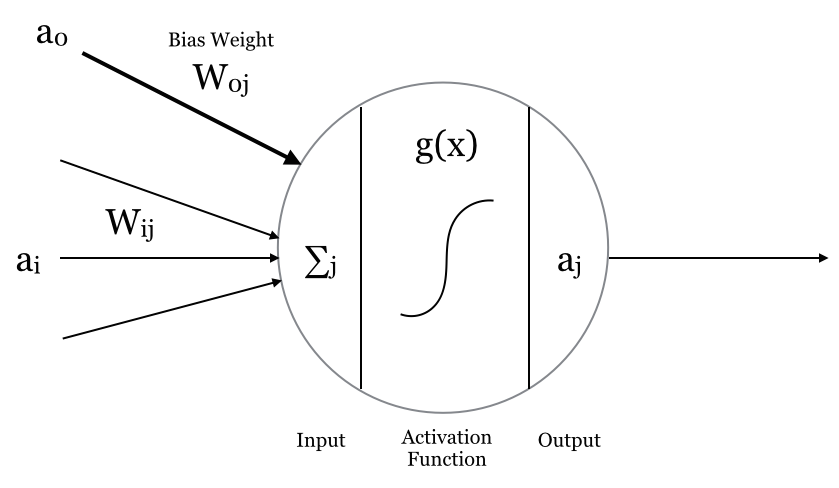
\includegraphics[width=0.4\textwidth]{diagrams/perceptron/perceptron.png}
\caption{Diagram of a basic perceptron units of a neural network. The weighted input of the training data is passed through an activation function to produce an output vector. Based on the diagram by Russell and Norvig \cite{russell1995artificial}.}
\label{fig:perceptron}
\end{figure}

Training neural networks is typically performed using the back-propagation algorithm \cite{lecun2012efficient}. Back-propagation first computes the error between the actual and expected output for a given training example in the final layer. The error in previous layers can be computed by ``back-propagating'' the error backwards from the final layer towards the input \cite{nnanddeeplearning}. More formally, the error in the final layer $L$ is given in matrix form by:

\begin{equation}
\label{eq:backprop1}
	\bm{\delta}^L = \nabla_a C \odot g'(\bm{z}^L)
\end{equation}

Where $\bm{\delta}^L$ is the error in the final layer, $\nabla_a C$ is the vector of partial derivatives of the cost $C$ function (typically quadratic cost or cross-entropy), $\bm{z}^L$ is the weighted vector of inputs to the final layer ($\bm{W}^L\bm{a}^{L-1}$), and $\odot$ is the Hadamard product. The vector $\bm{\delta}^L$ is then used to compute the error in previous layers as follows:

\begin{equation}
\label{eq:backprop2}
	\bm{\delta}^l = ((\bm{W}^{l+1})^T \delta^{l+1} \odot g'(\bm{z}^l)
\end{equation}

Once the gradient vectors $\bm{\delta}^l$ have been computed for every layer in the network the weights can be updated using an optimisation algorithm. The simplest optimisation approach is gradient descent \cite{lecun2012efficient}. In gradient descent the weights for each layer are updated according to:

\begin{equation}
	\bm{W}^l \leftarrow \bm{W}^l - \alpha \bm{\delta}^l
\end{equation}

Where $\alpha$ is parameter controlling the step size and in the simplest implementation is $\alpha$ is a constant. Alternative approaches can make use of Newton or Quasi-Newton methods \cite{lecun2012efficient}. Gradient descent training can either preformed in ``batches'' where the update is the sum of the error over all training examples, or stochastically after each example.

\begin{figure}[h!]
\centering
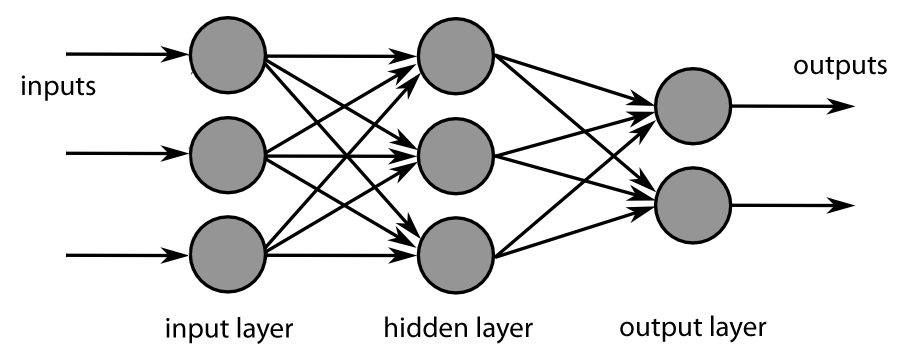
\includegraphics[width=0.4\textwidth]{diagrams/network.png}
\caption{Diagram of a very simple fully connected neural network architecture. The connections between the nodes are represented using the weight matrix $\bm{W}$. Each node is an activation function for a single element in the weighted input vector $\bm{z}^l$. Image source: \cite{multilayernetwork}}
\label{fig:neural-network}
\end{figure}


The basic architecture of a classical neural network is structured so that every node in one layer is connected to every node in the next via the weight matrix. This architecture is known as a ``fully connected'' network. Fully connected networks are feasible on a small scale. However, the complexity of a network rapidly grows in proportion on the size of the training examples and the number of layers used. This particularly becomes an issue when attempting to process very high dimensional data such as images.

Subsequently, much of the current research in neural networks is focused on the reducing the complexity of the architecture and the number of weight parameters used. Denil et al. \cite{denil2013predicting} demonstrated that there is a significant amount of redundancy in the parameterisation of neural networks. By reducing the number of parameters used or simplifying the architecture of the neural networks it is hoped that significant gains in time and memory complexity can be achieved. A reduction in network parameters also leads to a model that is potentially easier to train as there are less ``knobs'' to turn in order to fine tune the network.

There have been several notable prior methods to compress neural networks. In the simplest sense, the driving intuition behind convolutional neural networks \cite{krizhevsky2012imagenet} is that weights are effectively tied for a receptive field, forcing the network to only learn locally connected features. This combined with pooling layers \cite{zeiler2013stochastic} forms an architectural approach to parameter sharing. Early techniques such as ``Optimal Brain Damage'' by LeCun et al. \cite{lecun1989optimal} looked at the effect of removing parameters after training from a network based on the second order derivative. Nowlan \& Hinton \cite{nowlan1992simplifying} experimented with soft weight sharing with Gaussian mixtures as part of weight regularisation. More recently Srivastava et al. \cite{srivastava2014dropout} proposed Dropout for probabilistically dropping weights.

In the remainder of this paper we will examine three recent papers ($\textless 3$ years old) each taking a different approach to the problem of reducing the complexity of neural networks. Specifically we shall critique the work of Chen et al. on \textit{HashedNets} \cite{chen2015compressing}, Han et al. on ``\textit{Learning both Weights and Connections for Effcient Neural Networks}'' \cite{han2015learning}, and Denil et al. on \textit{Low-Rank Decomposition} \cite{denil2013predicting}.

\section{HashedNets}
\label{sec:hashednets}

\subsection{Research Undertaken}
\textit{HashedNets} by Chen et al. \cite{chen2015compressing} uses random weight sharing between layers in order to reduce the number of connections and utilises a hash function in order to avoid additional memory overheads and to automatically pool weights. 

More formally, in their design, the connections between each layer is represented by a ``virtual'' weight matrix $\bm{V}^l$ in which the elements of each matrix are mapped to a vector of real weights $\bm{w}^l$ containing $K$ elements where $K \ll N$ and where $N$ is the total number of connections between layers. The connections are mapped from $\bm{V}^l$ to $\bm{w}^l$ using a hash function $\phi : \mathbf{R}^m \rightarrow \mathbf{R}^n$. Weights are pooled by taking advantage of the fact that hash collisions will happen when $K \textless N$. This has the effect of allowing a virtual number of parameters to be represented using only a $K$ sized vector. Theoretically the size of $\bm{V}^l$ may be increased or decreased while the memory footprint of the network remains the same.

 The mapping from the virtual matrix to the actual weight vector causes the feed forward equation (equation \ref{eq:feedforward} in element wise form for just two layers) to be modified as follows:

\begin{equation}
	a_i = g(\sum_{j=1}^m V_{ij}a_j) = g(\sum_{j=1}^m w_{\phi(i,j)}a_j)
\end{equation}

Instead of using a hash function to transform $\bm{V}^l$ to $\bm{w}^l$ they hash the activation from the previous layer into a $K$ dimensional vector. This avoids the need for a matrix explicitly mapping virtual weights to real weights, saving memory. Therefore the final feed-forward equation becomes:

\begin{equation}
	a_i = g(\bm{w}^T \phi_i(\bm{a}))
\end{equation}

Where the hash function $\phi$ is defined as the sum of activations from the previous layer hashed into the $k^{th}$ bucket. The authors provide a proof that the two formulations are equivalent in \cite{chen2015compressing}. 

Additionally, and perhaps most importantly, the authors provide a derivation of a modified version of the back-propagation equations (equations \ref{eq:backprop1} and \ref{eq:backprop2}) which we have omitted here for brevity.

\begin{figure}[h!]
\centering
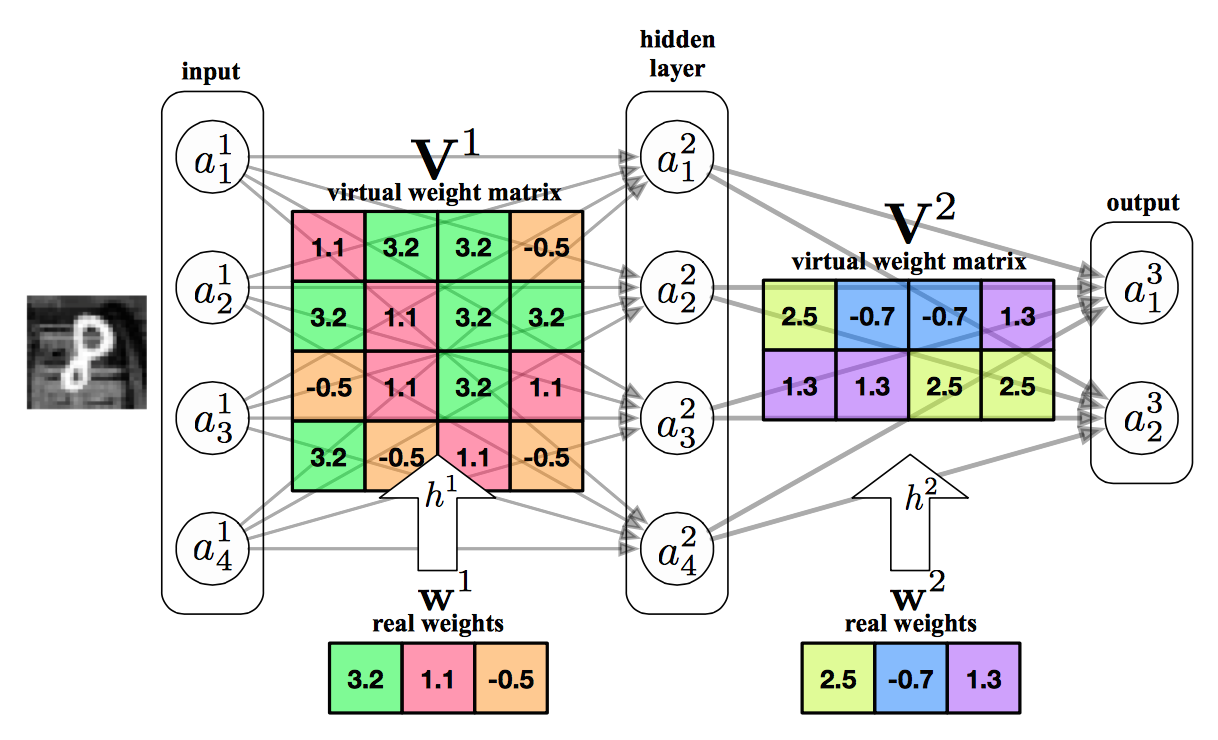
\includegraphics[width=0.5\textwidth]{diagrams/hashnets.png}
\caption{Conceptual view of the relationship between virtual and weights in \textit{HashedNets}. In practice it is the inputs which get hashed. Image source: \cite{chen2015compressing}}
\label{fig:hashednets}
\end{figure}


\subsection{Critique of Research}
Chen et al. clearly show that they have formulated a neural network architecture that can reduce the actual number of parameters used by a neural network by exploiting the hashing trick. While the method has its limitations, some of which are listed by the authors themselves, none are significant enough to render the study irrelevant. The results of the study are quite promising, providing good results in contrast to baseline methods with a design that is both easy to understand and implement.
 
They begin by clearly stating the motivation for their research by relating it to one of the major challenges facing modern neural network: the complexity of the models needed to work with modern datasets. Their justification for their specific direction of research is based on the work of Denil et al. \cite{denil2013predicting} who showed that there is a great deal of redundancy in neural network weight matrices. They argue that they can use the well known feature hashing trick to reduce this redundancy. Based on reading around this subject we would agree that this is both a fully justified motivation and sensible direction of research provided that compression gains are well balanced with the performance deterioration incurred by pooling weights.

The authors clearly state the method they used to implement feature hashing along with the relevant mathematical mechanics. Specifically, they provide two key derivations: firstly the show how the hashing function can be conceptually flipped from the hashing weights to hashing the activation output. Secondly they provide a derivation of the modified back propagation algorithm with the hash function included, necessarily proving that the network still can be trained conventionally. The derivations and their accompanying explanations are clear and accessible to the reader.

There are several limitations mentioned by the authors about their method which should be noted but are not significant enough for the method to not be useful in some dimension. The first is that feature hashing works best on sparse input where many features will be zero. The authors therefore encourage this by using ReLUs in activation. While these units are frequently used in modern NN approaches it would be interesting to see the effect of using a sigmoid function or very dense data and seeing how much this reduces the benefit of compression. Although this may be limited more by the ability to successfully train the network with different activations than by the compression technique.

Another limitation mentioned by the authors is that they have not managed to optimise their approach for GPU architectures where random memory access imposed by hash functions becomes an issue. It is noted that one of the authors is a NVIDIA employee which perhaps lowers the bias of the authors in relation to their own opinion as to how limiting this criticism is. Lack of an efficient GPU implementation is a major limiting factor for this methodology. However, if the parameter reduction achieved is significant enough a drop in GPU efficiency might be offset.

In the results of the paper the authors clearly demonstrate that their method out performs or is comparable to \textit{Low-Rank Decomposition} \cite{denil2013predicting} and \textit{Random Edge Removal} \cite{cirecsan2011high} over all chosen datasets and compression factors. It would have been better if they had provided some additional results regarding the training or convergence time compared to a standard network. This would give a sense of if it is more difficult to train compared to a standard approach or even if the methodology actually accelerates learning.

Importantly the datasets used are all variations well known neural network community. Specifically they use MNIST \cite{lecun1998gradient} and a couple of variations \cite{larochelle2007empirical} and two artificial datasets CONVEX and RECT \cite{larochelle2007empirical}. However, this study could of perhaps gone further in this area and experimented with a more challenging real world natural image dataset such as CIFAR-10 \cite{krizhevsky2009learning} or ImageNet \cite{deng2009imagenet}. This would of given some results for a more realistic real world yard stick in comparison with the fairly dated MNIST. They could have also combined complex image datasets with different types of layers (i.e. convolution) with hashed layers for more practical performance results. Additionally, it would have been nice to see some results on larger architectures or commonly used models such as those that are available in Caffe \cite{jia2014caffe}.

Their choice to produce results combined with the ``Dark Knowledge'' approach of Hinton et al. \cite{hinton2015distilling} is quite interesting. The results of their experiments show that best result were achieved using the combination of feature hashing and a distilled model. The difference between the vanilla HashNet and a joined model is not hugely significant. However, this does show a good example of how the author's methodology lends itself to being combined with alternative approaches.

\section{Pruning Connections and Neurons}
\label{sec:pruning}

\subsection{Research Undertaken}
In their recent paper Han et al. \cite{han2015learning} propose a simple technique to enable a neural network to learn sparse connectivity between neurons. The high level view of their methodology is to initially train a large network, then prune weights which only contribute a small amount using a threshold parameter. Neurons which are left with no incoming or outgoing connections are removed from the network. The pruning and retraining phases are repeated many times in order to find the minimum number of connections required by the network. In the experiments described the pruning threshold was chosen to be a parameter multiplied by the standard deviation of the layer's weights.

To prevent over-fitting during the retraining stages the authors made use of the Dropout \cite{srivastava2014dropout} technique. The authors note that they must make an adjustment to the dropout ratio due to the ``hard pruning'' effect in the connection pruning phase. The authors suggest a derivation for the ratio, suggesting the correct dropout rate is proportional to the square root of the quotient of connections to a layer before and after pruning.

\begin{figure}[h!]
\centering
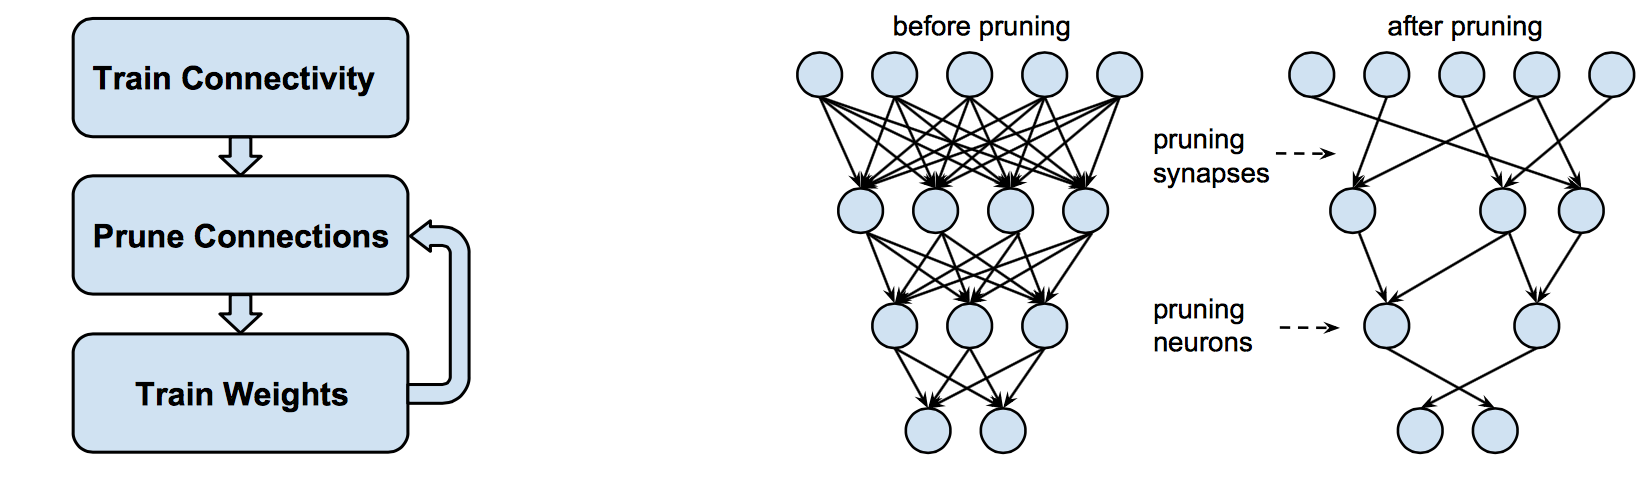
\includegraphics[width=0.48\textwidth]{diagrams/iterative-pruning.png}
\caption{Left: Overview of the iterative pruning approach. Right: How connectivity is leant, first weights are dropped, then neurons. Image source: \cite{han2015learning}}
\label{fig:iterative-pruning}
\end{figure}

The authors also experimented, based on prior literature and their own research, with a couple of implementation specifics to give optimum results in their own tests. L2 regularisation was shown to be the best choice overall despite L1 regularisation giving better accuracy after the pruning phase (as it forces more weights towards zero). The authors also make the case that training the network from the surviving parameters rather than reinitialising trained layers produces better results. This also has the advantage that only the pruned layers need to be retrained, which can be done using regular back propagation.

\subsection{Critique of Research}
Han et al. \cite{han2015learning} show that they have developed an effective method of training a NN to produce a sparse architecture with solid and verifiable results to back their conclusions.

Their proposed method is based on the prior work of Srivastava et al. \cite{srivastava2014dropout} but modified so that weights cannot be brought back into existence once dropped. Some of the subsections outlining the methodology they used appears to be a little terse in places. In particular subsection 3.3 could use expansion and possibly a diagram to more clearly express their method and their justification for the retraining procedure.

The authors clearly show that they have a method of achieving excellent compression vs. test accuracy rates compared to recent competing methods in the field. They carried out all of their experiments using the well known NN framework Caffe \cite{jia2014caffe} and used reference models making their methodology easier to validate in comparison with \textit{HashedNets}. The authors show strong compression results across several different well known network implementations across two datasets. Beginning with MNIST \cite{lecun1998gradient} the authors show compression rates of up to 12x for LeNet-300-100 and LeNet-5 with only a small ($< 0.06$) drop in accuracy. As well as testing on MNIST, the authors show good compression results on the more complex ImageNet database \cite{deng2009imagenet}.

A higher compression vs. test error rate seems likely compared with a effectively random technique such as \textit{HashedNets} because they are training the network to lose only irrelevant parameters. In other words they can achieve a high compression rate and high test accuracy because they are making a choice about which weights to keep. This is better than choosing at random which is the case with \textit{HashedNets}. This is reflected in the deterioration in accuracy seen in the 5 layer versions of HashNets where a larger network could lead to randomly pooling weights having a greater attenuation effect across layers.

A strong advantage to this methodology over approaches such as \textit{HashedNets} is that the level of compression is automatically chosen by the algorithm. Only the hyper-parameter controlling the pruning threshold need be selected, either globally or layer by layer. This means that the technique is perhaps easier to tune that other approaches. This could also be interpreted as a weakness because the rate of compression is effectively heavily dependant on the sparsity of the data which will change between datasets.

A major limitation of this approach in comparison with that of \textit{HashedNets} in section \ref{sec:hashednets} is a full, ``uncompressed'' neural network must first be trained, then pruned and retrained instead of starting at a smaller size initially. If the network needs to be constrained with restricted memory then this approach would not work. This is a big issue for extremely large networks where a distributed implementation is required in order to train them. If the purpose of reducing the number of parameters so that the network may be trained on a single machine then this method may not be appropriate. Using this approach also requires the network to be retrained after the pruning stage, while in contrast \textit{HashedNets} are simply trained in a compressed state.

One element of the paper which was particularly insightful was the visualisation of a layer's sparsity pattern. NNs are notorious black boxes and this paper contributed an interesting visualisation of a layer's sparsity and linked it with the characteristics of the MNIST dataset. Such techniques may be helpful in understanding of a dataset and tweaking the design of a NN accordingly.

\section{Low-Rank Decomposition}

\subsection{Research Undertaken}
Denil et al. \cite{denil2013predicting} illustrate an approach to compression known in literature as \textit{Low-Rank Decomposition}. The basic principle behind their methodology is to take the weight matrix $\bm{W}$ and decompose the matrix into two smaller matrices:

\begin{equation}
\label{eq:low-rank}
	\bm{W} = \bm{UV}
\end{equation}

Where $\bm{U}$ has the same number of rows as the input vector $\bm{a}^{l-1}$ and $\bm{V}$ has the same number of columns as the size of the output vector $\bm{a}^{l}$. The remaining dimension $n_\alpha$ (the columns of $\bm{U}$ and the rows of $\bm{V}$) determines the level of compression. The smaller $n_\alpha$ becomes the less effective parameters a layer has. 

\begin{figure}[h!]
\centering
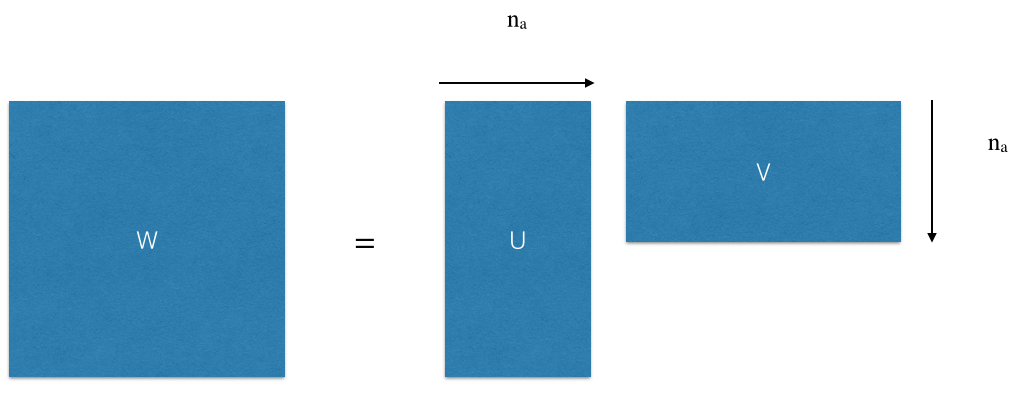
\includegraphics[width=0.5\textwidth]{diagrams/low-rank.jpg}
\caption{Visualisation of the decomposition of the weight matrix $\bm{W}$ into two smaller matrices $\bm{U}$ and $\bm{V}$}
\label{fig:low-rank}
\end{figure}


In their method they propose to fix the value of $\bm{U}$ and let only $\bm{V}$ be learned. This intuitively makes sense because the two matrices will still have redundancies as they are both linear combinations of each other. Subsequently the matrix $\bm{U}$ can be chosen to be a matrix where the columns are bases for $\bm{V}$. The rest of their methodology concerns finding good choices for $\bm{U}$.

The authors present a number of different methods for choosing the columns of $\bm{U}$. One choice is to randomly choose columns for the identity function which equates to just picking random connections. Another is to choose the  columns to be random unit vectors orthogonal to each other, as in random projections. They also present more advanced choices that encode prior knowledge about the feature space through the use of a kernel. Complex features are shown to be predicted using the kernel ridge predictor \cite{welling2013kernel}:

\begin{equation}
\label{eq:ridge-predictor}
	\bm{w} = \bm{k_\alpha}^T(\bm{K_\alpha} + \lambda I)\bm{w_\alpha}
\end{equation}

The preceding equation is predicting a single column $\bm{w}$ of the final weight matrix $\bm{W}$ given a subset of the original weight vector $\bm{w_\alpha}$. Note that this can be parallelised by giving multiple example inputs as a matrix $\bm{W_\alpha}$. Equation \ref{eq:ridge-predictor} can be also be intuitively broken apart and equated to $\bm{U}$ and $\bm{V}$:

\begin{equation}
	\bm{U} = \bm{k_\alpha}^T(\bm{K_\alpha} + \lambda I)
\end{equation}
\begin{equation}
	\bm{V} = \bm{w_\alpha}
\end{equation}

The choice of kernel function used for $\bm{k_\alpha}$ and $\bm{K_\alpha}$ are experimented with as part of the author's research. For example, in the case of an image this could be the Gaussian radial basis kernel. They also show that construction of the kernel also be inferred by the data by training a layer as an autoencoder. 

\begin{figure}[h!]
\centering
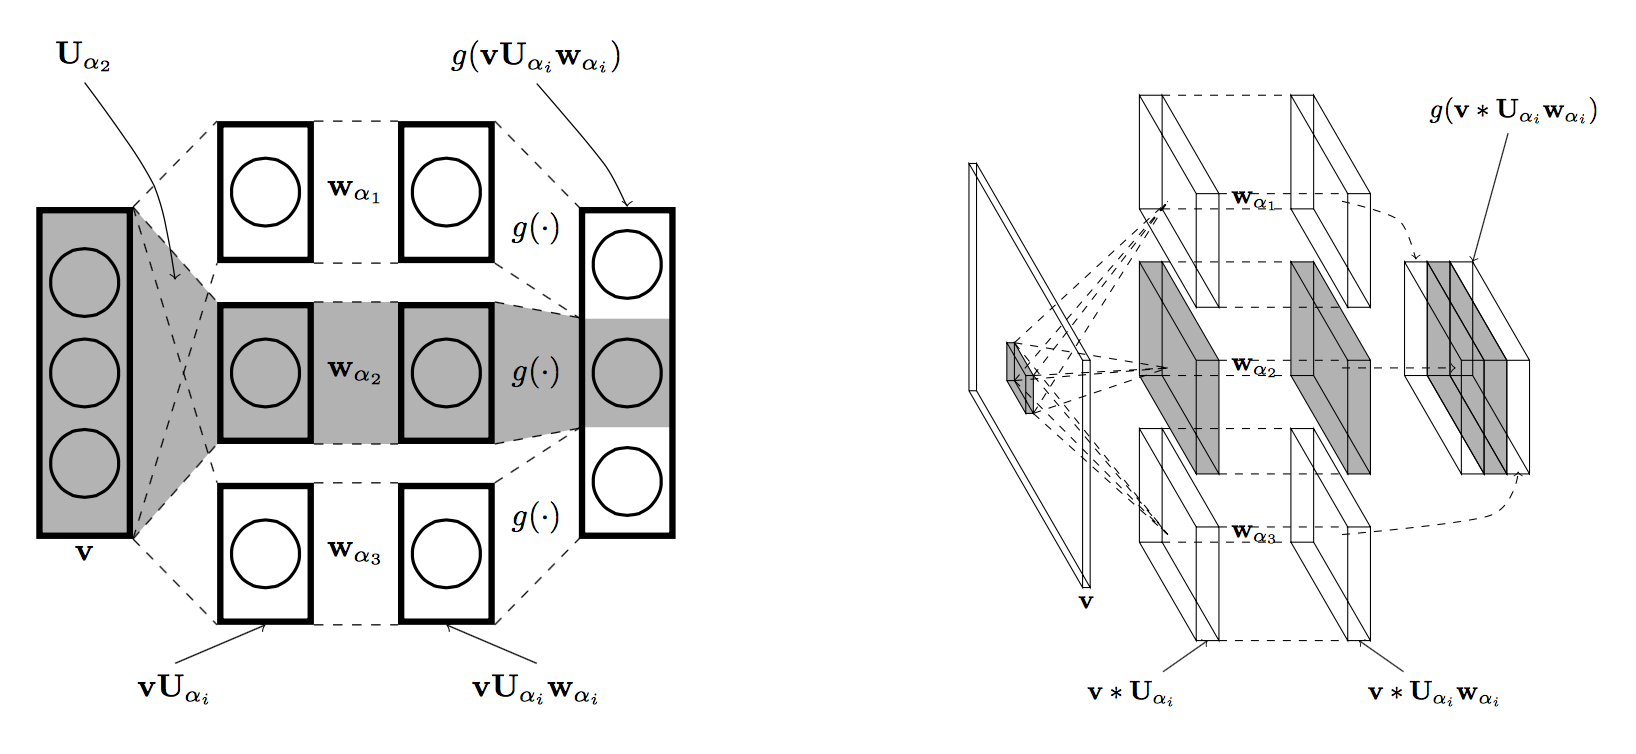
\includegraphics[width=0.5\textwidth]{diagrams/low-rank-columns.png}
\caption{Columnar architecture of a fully connected (left) and convolutional (right) network. Each column corresponds to a different set of weight indices ($\alpha$). Image source: \cite{denil2013predicting}}
\label{fig:low-rank-columns}
\end{figure}

The authors also propose an architectural structure (figure \ref{fig:low-rank-columns}) in which multiple basis dictionaries can be be used in the case that one such dictionary is too restrictive. They propose that a sub matrix $\bm{U}_{\alpha j}$ can be created and used to predict the a corresponding feature matrix $\bm{W}_j = \bm{U}_{\alpha j} \bm{W}_{\alpha j}$ where $j \in J$ is the index of the number of sub matrices. Each sub matrix can then be concatenated to produce the final matrix $\bm{W}$.

\subsection{Critique of Research}
Denil et al. \cite{denil2013predicting} show a flexible solution for reducing the parameters of a neural network using matrix decomposition in an influential paper that also showed that NN weights have a great deal of redundancy.

One of the biggest strengths of this technique, outlined by the authors, is that the formulation is independent of many of the peripheral choices when designing a neural network architecture. The performance of their approach is not dependant on the activation function, choice of regularisation, architecture of layers etc. This is very useful both because it means that the technique is likely to be applicable to a wide variety of practical uses. This also makes it readily applicable to being combined with other compression approaches.

A major advantage in contrast with techniques like the one presented in section \ref{sec:pruning} is that, like \textit{HashedNets}, a the network is trained with the compressed representation. A full neural network is never grown at any point. This means it is suitable for making a very large network small enough to be trained on a single physical machine and could avoid the need for a distributed architecture.

The choice of the basis dictionary $\bm{U}$ in their formulation is highly flexible. The authors propose a number of different approaches for choosing $\bm{U}$. This means that given a specific neural network $\bm{U}$ can be tailored to its requirements using methods such as kernel ridge regression and pre-training layers as autoencoders. However, this is also a weakness of the method because it adds an additional number of choices we must make about our system. The question: ``what basis dictionary is best for my input?'' is not trivial to answer and highly dependant on the dataset. Additionally, the choice of indices ($\alpha$) used suffers from the same problems. The authors propose just choosing randomly, but if we wish to do better than this we must carefully formulate a selection criteria, which is again likely to be data specific.

While the proposed method is perhaps not the easiest choice to work with in practice, their paper did show a high level of redundancy in the parameters of both fully connected and convolutional neural networks. Based on their results they provide a strong and enjoyable write up of future directions of research.

The results of the paper are detailed and interesting. The authors provide several different implementations of their design using different basis dictionaries and showed how almost all of them can be trained to give good performance compared to a conventional network. The fact that the authors used two common datasets (MNIST and CIFAR-10) makes their results easily verifiable. It was also encouraging to see results of their approach combined with an alternative architecture (i.e. convolutional), showing that the approach will work with other architectures.

In terms of the papers discussed here, the authors of \textit{HashedNets} directly compared their approach with the low rank approach presented in this section. It is worth noting that low-rank decomposition was shown to be inferior to the plain \textit{HashedNets} implementation. The authors of \textit{HashedNets} used a zero-mean Gaussian distribution as their fixed matrix. However, it may be the case that a better choice for the basis dictionary would of yielded better results over a relatively naive Gaussian distribution implementation. 




% needed in second column of first page if using \IEEEpubid
%\IEEEpubidadjcol

% An example of a floating figure using the graphicx package.
% Note that \label must occur AFTER (or within) \caption.
% For figures, \caption should occur after the \includegraphics.
% Note that IEEEtran v1.7 and later has special internal code that
% is designed to preserve the operation of \label within \caption
% even when the captionsoff option is in effect. However, because
% of issues like this, it may be the safest practice to put all your
% \label just after \caption rather than within \caption{}.
%
% Reminder: the "draftcls" or "draftclsnofoot", not "draft", class
% option should be used if it is desired that the figures are to be
% displayed while in draft mode.
%
%\begin{figure}[!t]
%\centering
%\includegraphics[width=2.5in]{myfigure}
% where an .eps filename suffix will be assumed under latex, 
% and a .pdf suffix will be assumed for pdflatex; or what has been declared
% via \DeclareGraphicsExtensions.
%\caption{Simulation Results}
%\label{fig_sim}
%\end{figure}

% Note that IEEE typically puts floats only at the top, even when this
% results in a large percentage of a column being occupied by floats.


% An example of a double column floating figure using two subfigures.
% (The subfig.sty package must be loaded for this to work.)
% The subfigure \label commands are set within each subfloat command, the
% \label for the overall figure must come after \caption.
% \hfil must be used as a separator to get equal spacing.
% The subfigure.sty package works much the same way, except \subfigure is
% used instead of \subfloat.
%
%\begin{figure*}[!t]
%\centerline{\subfloat[Case I]\includegraphics[width=2.5in]{subfigcase1}%
%\label{fig_first_case}}
%\hfil
%\subfloat[Case II]{\includegraphics[width=2.5in]{subfigcase2}%
%\label{fig_second_case}}}
%\caption{Simulation results}
%\label{fig_sim}
%\end{figure*}
%
% Note that often IEEE papers with subfigures do not employ subfigure
% captions (using the optional argument to \subfloat), but instead will
% reference/describe all of them (a), (b), etc., within the main caption.


% An example of a floating table. Note that, for IEEE style tables, the 
% \caption command should come BEFORE the table. Table text will default to
% \footnotesize as IEEE normally uses this smaller font for tables.
% The \label must come after \caption as always.
%
%\begin{table}[!t]
%% increase table row spacing, adjust to taste
%\renewcommand{\arraystretch}{1.3}
% if using array.sty, it might be a good idea to tweak the value of
% \extrarowheight as needed to properly center the text within the cells
%\caption{An Example of a Table}
%\label{table_example}
%\centering
%% Some packages, such as MDW tools, offer better commands for making tables
%% than the plain LaTeX2e tabular which is used here.
%\begin{tabular}{|c||c|}
%\hline
%One & Two\\
%\hline
%Three & Four\\
%\hline
%\end{tabular}
%\end{table}


% Note that IEEE does not put floats in the very first column - or typically
% anywhere on the first page for that matter. Also, in-text middle ("here")
% positioning is not used. Most IEEE journals use top floats exclusively.
% Note that, LaTeX2e, unlike IEEE journals, places footnotes above bottom
% floats. This can be corrected via the \fnbelowfloat command of the
% stfloats package.







% if have a single appendix:
%\appendix[Proof of the Zonklar Equations]
% or
%\appendix  % for no appendix heading
% do not use \section anymore after \appendix, only \section*
% is possibly needed

% use appendices with more than one appendix
% then use \section to start each appendix
% you must declare a \section before using any
% \subsection or using \label (\appendices by itself
% starts a section numbered zero.)
%


%\appendices
%\section{Proof of the First Zonklar Equation}
%Some text for the appendix.

% use section* for acknowledgement
%\section*{Acknowledgment}
%
%
%The authors would like to thank...


% Can use something like this to put references on a page
% by themselves when using endfloat and the captionsoff option.
\ifCLASSOPTIONcaptionsoff
  \newpage
\fi



% trigger a \newpage just before the given reference
% number - used to balance the columns on the last page
% adjust value as needed - may need to be readjusted if
% the document is modified later
%\IEEEtriggeratref{8}
% The "triggered" command can be changed if desired:
%\IEEEtriggercmd{\enlargethispage{-5in}}

% references section

% can use a bibliography generated by BibTeX as a .bbl file
% BibTeX documentation can be easily obtained at:
% http://www.ctan.org/tex-archive/biblio/bibtex/contrib/doc/
% The IEEEtran BibTeX style support page is at:
% http://www.michaelshell.org/tex/ieeetran/bibtex/
%\bibliographystyle{IEEEtran}
% argument is your BibTeX string definitions and bibliography database(s)
%\bibliography{IEEEabrv,../bib/paper}
%
% <OR> manually copy in the resultant .bbl file
% set second argument of \begin to the number of references
% (used to reserve space for the reference number labels box)
\bibliographystyle{plain}
\bibliography{references}
%\begin{thebibliography}{1}
%
%\bibitem{IEEEhowto:kopka}
%H.~Kopka and P.~W. Daly, \emph{A Guide to \LaTeX}, 3rd~ed.\hskip 1em plus
%  0.5em minus 0.4em\relax Harlow, England: Addison-Wesley, 1999.
%
%\end{thebibliography}

% biography section
% 
% If you have an EPS/PDF photo (graphicx package needed) extra braces are
% needed around the contents of the optional argument to biography to prevent
% the LaTeX parser from getting confused when it sees the complicated
% \includegraphics command within an optional argument. (You could create
% your own custom macro containing the \includegraphics command to make things
% simpler here.)
%\begin{biography}[{\includegraphics[width=1in,height=1.25in,clip,keepaspectratio]{mshell}}]{Michael Shell}
% or if you just want to reserve a space for a photo:

%\begin{IEEEbiography}[{
\includegraphics[width=1in,height=1.25in,clip,keepaspectratio]{picture}}]{John Doe}
%\blindtext
%\end{IEEEbiography}

% You can push biographies down or up by placing
% a \vfill before or after them. The appropriate
% use of \vfill depends on what kind of text is
% on the last page and whether or not the columns
% are being equalized.

%\vfill

% Can be used to pull up biographies so that the bottom of the last one
% is flush with the other column.
%\enlargethispage{-5in}



% that's all folks
\end{document}


